\subsection{Object Manipulation}

\subsubsection{Motion Planning.}
RRTConnect~\cite{kuffner2000rrt} plans collision-free trajectories, keeping the end-effector upright while carrying an object to pour. To reduce collision-checking time, the planning scene uses simple primitives: RANSAC~\cite{martinez2022ransac} segments the table as an oriented box, and the target object is approximated by spheres fitted to its voxel-downsampled point cloud. The rest of the scene comes from an OctoMap built from the depth camera.

\subsubsection{Picking.}
Objects are segmented by fusing 2D detections with depth. Solid objects are fitted by RANSAC~\cite{martinez2022ransac} to a sphere, upright cylinder or cuboid. Sampled grasps that collide with the scene or exceed the gripper opening are discarded. The remainder candidate grasps are scored by spare aperture, closeness to the object's center and arm movement cost, the five highest-scored pre-grasp poses are in order validated through the motion planner with a Cartesian approach to close in. Grasp Pose Detection (GPD) ~\cite{ten2017grasp} handles shelf and pouring grasps and is the general fallback.

\subsubsection{Placing \& Pouring.}
Placing scores the whole table with Gaussian kernels that reward free space and penalize nearby objects and edges, multiplied by a directional map for spatial requests (e.g., ``in front of X'', Fig.~\ref{fig:manip}a); only front, back, left, right and ``close to'' are supported. For pouring, PCL~\cite{rusu20113d} estimates the container's rim height, and the object is tilted 15\,cm above it at a fixed angle, without feedback on the poured amount.

\subsubsection{Experimental Validation.}
We compared the geometric generator and GPD on the real robot, each without fallback to the other; an operator confirmed every outcome. Seven household objects were tested alone at five table positions (5 trials per method, up to 61\,cm from the arm base), and in five reproducible clutter scenes of 4--5 objects, rebuilt from reference images as in SceneReplica~\cite{khargonkar2024scenereplica}. Geometric grasps held significantly more often (Table~\ref{tab:manipulation_results}; McNemar $p=0.007$ alone, $p=0.012$ in clutter). The stack reported success in 24 of GPD's 36 failures, while the object was not held or was the wrong one. All 67 held objects were placed correctly on free surface. Detector misses (8) were excluded. Low, curved and thin objects remain weak (banana and spoon 1/5 each). Trial data: \href{https://github.com/RoBorregos/home2/tree/main/manipulation/benchmarks/2026-11}{\texttt{home2/manipulation/benchmarks}}.

\begin{table}[h]
\centering
\caption{Objects held on the real robot, and mean time per held object including failures.}
\label{tab:manipulation_results}
\begin{tabular}{lccc}
\toprule
\textbf{Scenario} & \textbf{Geometric} & \textbf{GPD} & \textbf{Time per hold (Geo / GPD)} \\
\midrule
Alone (7 objects) & 23/35 (66\%) & 12/35 (34\%) & 14.4 / 33.6\,s \\
Clutter (5 scenes) & 20/24 (83\%) & 11/24 (46\%) & 11.8 / 28.7\,s \\
\bottomrule
\end{tabular}
\end{table}

\subsubsection{Custom Gripper.}
FRIDA's low-cost, open-source\footnote{\url{https://grabcad.com/library/robotic-gripper-34}} parallel gripper is based on the UMI design~\cite{chi2024universal}: a high-torque servo drives the fingers through a rack and pinion, holding objects up to 1\,kg. The 3D-printed TPU fingers have an inner structure that deforms to complex geometries (Fig.~\ref{fig:manip}b).

\begin{figure}[H]
\centering
\begin{minipage}{0.19\textwidth}\centering
  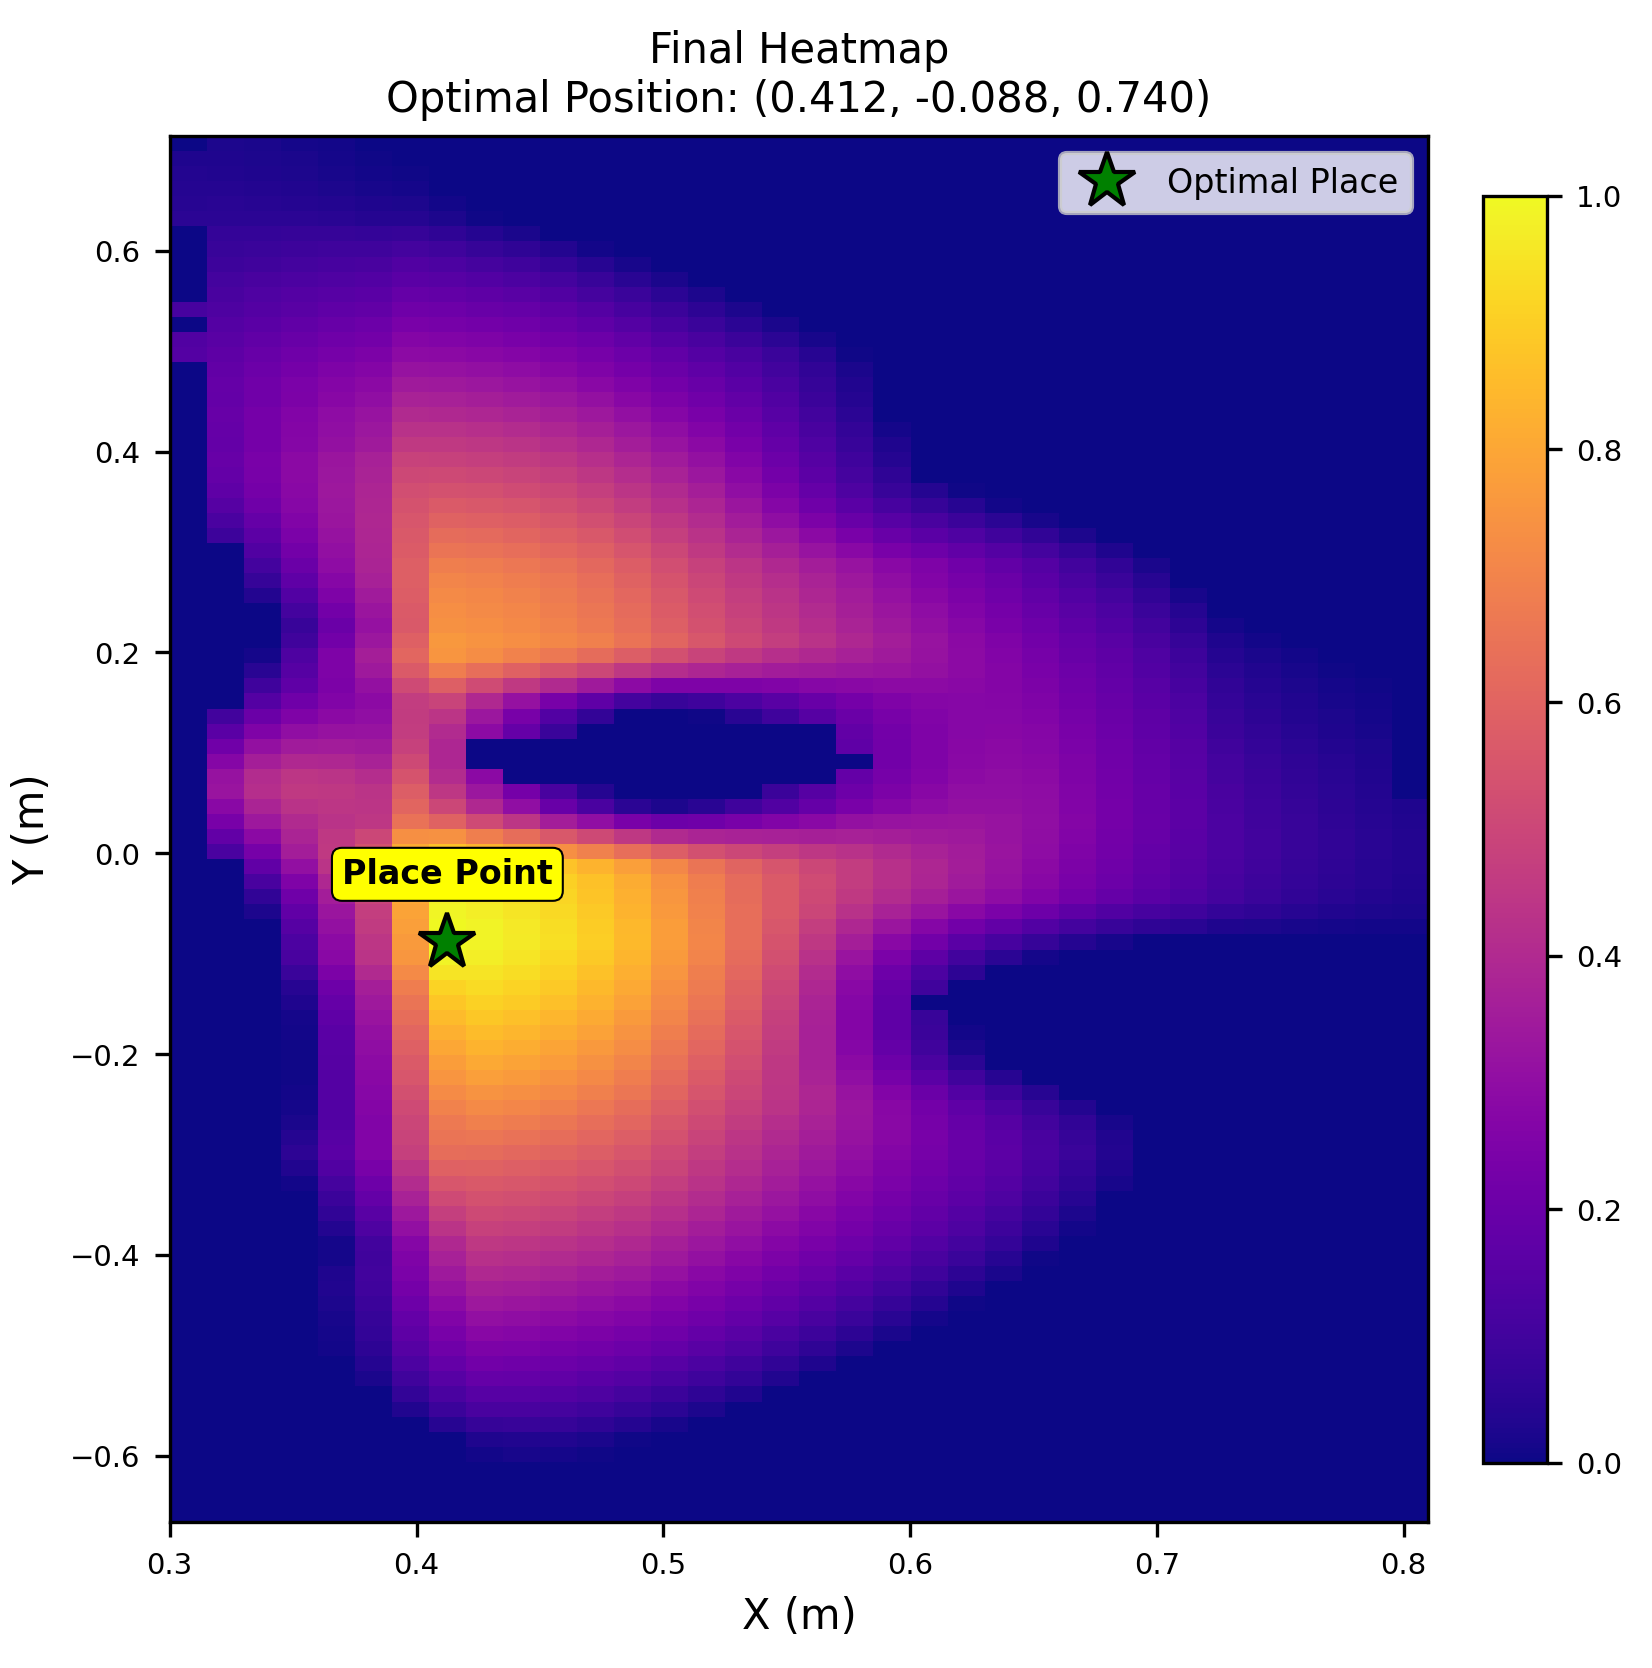
\includegraphics[width=\linewidth]{TDPTemplate-master/images/HeatMaps_2027_final.png}\\(a)
\end{minipage}\hfill
\begin{minipage}{0.43\textwidth}\centering
  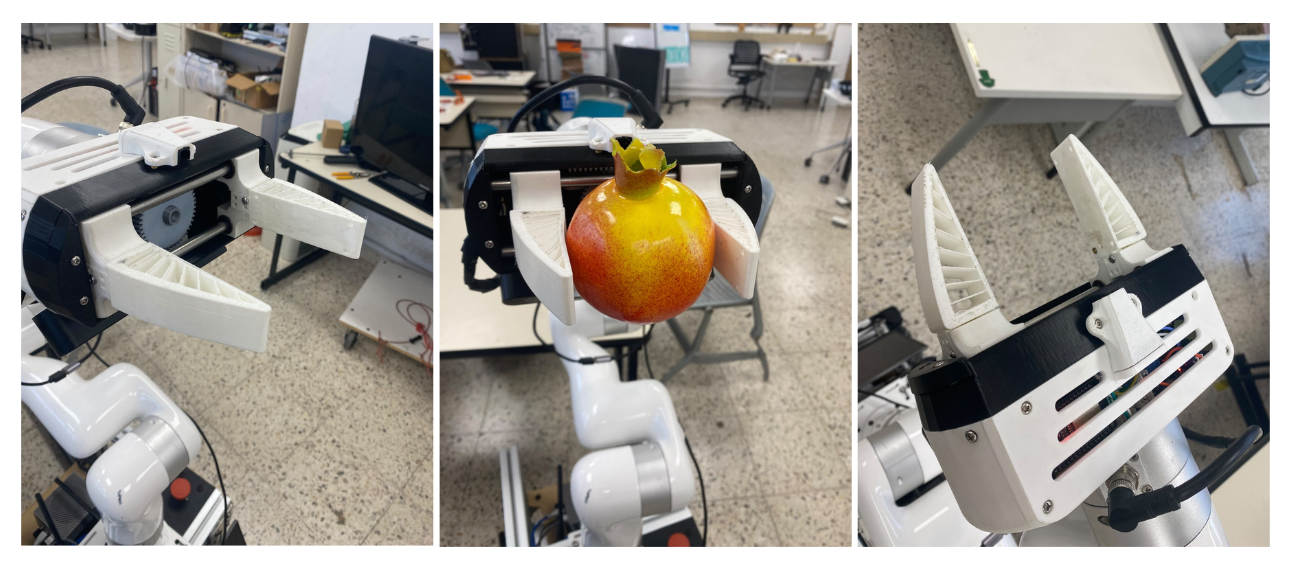
\includegraphics[width=\linewidth]{TDPTemplate-master/images/Gripper_Soft.png}\\(b)
\end{minipage}\hfill
\begin{minipage}{0.33\textwidth}\centering
  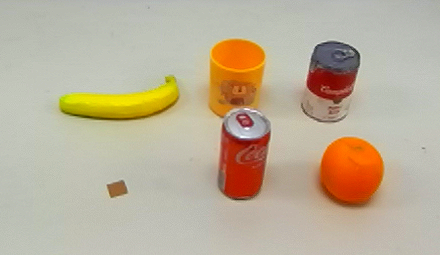
\includegraphics[width=\linewidth]{TDPTemplate-master/images/clutter_scene4.png}\\(c)
\end{minipage}
\caption{(a) Final placement heatmap for an ``in front of'' request. (b) Gripper grasps from different positions. (c) Clutter scene from the experiment.}
\label{fig:manip}
\end{figure}
